\chapter{Design}

Hyperledger Fabric and Composer will be used to design and implement blockchain solution. Firstly we have to become familiar with the technologies that Fabric provides and makes it easier to develop a product. 
During the design of the blockchain network on the Windows machine, I encountered a lot of time-consuming and annoying problems that were caused by Windows itself. Since the Hyperledger project is maintained by Linux Foundation it made sense to use a Linux operating system. Unfortunately, this decision caused another problem. A lot of companies in the automotive industry use windows based systems. The Windows Control and Automation Technology developed by Beckhoff is a software system that turns almost any compatible PC into a real-time controller with a multi-PLC system is also Windows-based and a place where most of the programs are run. To overcome this issue I installed Ubuntu to VirtualBox where the solution is deployed to. This design decision also enables portability and ease of deployment.

\section{Docker}
Docker is a computer program that performs operating-system-level virtualization. Docker is used to run software packages called containers. Containers are isolated from each other and bundle their own application, tools, libraries and configuration files; they can communicate with each other through well-defined channels. All containers are run by a single operating system kernel and are thus more lightweight than virtual machine \cite{docker}. Great benefit of docker is that it can be also run within the virtual machine in VirtualBox.It's using YAML markup language to define the configuration for Docker images. Very simple syntax and ease of use make it perfect to store configurations. Docker is used by Fabric to deploy peers and nodes as containers that can be easily run.

\section{Chaincode}
To implement chaincode on Fabric network I decided to use JavaScript because of the \emph{async await} keywords which can simplify asynchronous code and make it look like synchronous code. Chaincode is supposed to be simple and implement operations that all peers agreed on. During the instantiation process, the Peer uses Docker to run a container with the chaincode inside. The Peer is responsible for managing the chaincode container’s lifecycle and networking.


\section{Hyperledger Composer}

Hyperledger Composer is a programming model containing a modelling language, and a set of APIs to quickly define and deploy business networks and applications that allow participants to send transactions that exchange assets.

%\subsection{Blockchain State Storage}
%All transactions submitted through a business network are stored on the blockchain ledger, and the current state of assets and participants are stored in the blockchain state database. The blockchain distributes the ledger and the state database across a set of peers and ensures that updates to the ledger and state database are consistent across all peers using a consensus algorithm.

%\subsection{Connection Profiles}
%Hyperledger Composer uses Connection Profiles to define the system to connect to. A connection profile is a JSON document the is part of a business network card. These profiles are usually provided by the creator of the system they refer to and should be used to create business network cards in order to be able to connect to that system.

\subsection{Assets}
Assets are tangible or intangible goods, services, or property, and are stored in registries. Assets can represent almost anything in a business network, for example, a house for sale, the sale listing, the land registry certificate for that house, and the insurance documents for that house may all be assets in one or more business networks.

Assets must have a unique identifier, timestamp and provide a way to store any data in it. To solve the issue of a frequently changed data structure of manufacturing data, I decide to provide \emph{data} field which should be used for JSON values that are already being stored in NoSQL

\subsection{Participants}

Participants are members of a business network. They may own assets and submit transactions. Participant types are modelled, and like assets, must have an identifier and can have any other properties as required.

Participants in our network will be identified as companies with an id and name. 

\subsection{Identities}
An identity is a digital certificate and private key. Identities are used to transact on a business network and must be mapped to a participant in the business network. A single identity is stored in a business network card and if that identity has been mapped to a participant, it allows the user of that business network card to transact on a business network as that participant.

Identities will consist of two customers accessing the network. Besides network admin card a user card has to be specified for every single organisation in the network.

\subsection{Business Network cards}

Business network cards are a combination of an identity, a connection profile, and metadata, the metadata optionally containing the name of the business network to connect to. Business network cards simplify the process of connecting to a business network and extend the concept of an identity outside the business network to a 'wallet' of identities, each associated with a specific business network and connection profile.

\subsection{Transactions}

Transactions are the mechanism by which participants interact with assets. This could be as simple as a participant placing a bid on an asset in an auction. What we care about in this 
Queries

Transactions in the network will represent a change of the ownership of the product. Once the product has created it should belong to the domain owner \emph{mts.sk}. As soon as the product is assembled his ownership will be transferred to the different participant on the network - to another company. After shipment of the product, the ownership should be changed to the company which has ordered the product so we can verify what state product left the manufacturer.

\section{Historian registry}
The historian is a specialised registry which records successful transactions, including the participants and identities that submitted them. The historian stores transactions as \emph{HistorianRecord} assets, which are defined in the Hyperledger. 
This asset should be used as a logging mechanism.


\section{Hyperledger Fabric Architecture}

To understand Hyperledger Fabric's architecture we have to describe underlying concepts that are part of the system.

\begin{description}

\item[Domain] is the top-level namespace for the project. Usually, the project name or the domain name is used as the Hyperledger Fabric’s domain.


\item[Orderers] exist under a domain, there are orderers who are responsible for making sure that all the peers in the network have committed a transaction. When a transaction is proposed and committed by a peer, the orderer is informed about the new transaction and it forwards and commits this block to all adjacent peers. Orderer p is responsible for consistent Ledger state across the network

\item[Certificate authorities] are responsible for handling all the access control logic, issuing the identities and permission for the users in the Hyperledger blockchain network. To connect the network every peer needs to obtain an enrollment certificate from   CA. It authorises a peer to connect to the network and to acquire transaction certificates, which are needed to submit transactions. 

\item[Peers] are nodes which are connected to clients and are responsible for committing transactions to the world state. Each peer has its own copy of transactions in a CouchDB database. An organization can have more than one peer. Though it is advised to have multiple peers in an orderer to avoid data loss, having more than 3 or 4 peers might result in higher latency rates.

\item[Organization] is a managed group of members. Each member organization in the blockchain network is responsible to setup their peers for participating in the network. All of these peers need are configured with appropriate cryptographic materials like Certificate Authority.

\end{description}

On a Hyperledger Fabric network, the flow of data for queries and transactions is initiated by a client-side application by submitting a transaction request to a peer on a channel. The initial flow of data across the network is common to both queries and transactions. Using API available in the SDK, a client application signs and submits a transaction proposal to the appropriate endorsing peers on the specified channel. This initial transaction proposal is a request for endorsement. Each peer on the channel verifies the identity and authority of the submitting client, and (if valid) runs the specified chaincode against the supplied inputs. Based on the transaction results and the endorsement policy for the invoked chaincode, each peer returns a signed YES or NO response to the application. Each signed YES response is an endorsement of the transaction.
At this point in the transaction flow, the process diverges for queries and transactions. If the proposal called a query function in the chaincode, the application returns the data to the client. If the proposal called a function in the chaincode to update the ledger, the application continues with the following steps: The application forwards the transaction, which includes the read/write set and endorsements, to the ordering service. The transaction is then relayed to the ordering service. All channel peers validate each transaction in the block by applying the chaincode-specific Validation Policy and running a Concurrency Control Version Check.
Any transactions that fails the validation process are marked as invalid in the block, and the block is appended to the channel's ledger \cite{transaction_flow}. All valid transactions update the state database accordingly with the modified key/value pairs.

\begin{figure}[H]
    \begin{center}
        \begin{minipage}{\linewidth}
            \begin{center}
                \shadowimage[width=(\textwidth),keepaspectratio]{img/transaction_flow.png}
                \caption{Fabric transaction flow }
                \label{obr 1.2.1}
            \end{center}
        \end{minipage}
    \end{center}
\end{figure}

For the purpose of re-use of our blockchain network for multiple projects, I decided for following naming and topology. Domain should always be the name of the company under which this network has been developed. Organisations will start with generic name \emph{org} because we don't know which companies will be willing to join this network. Each organisation in the consortium will have its own certificate authority and two peers to create trust in the network. Since data is the property of customer using the service we will have more instances of the network. 

\newpage
\begin{itemize}
  \item \textbf{Domain} mts.sk
  \item \textbf{Orderer} orderer.mts.sk
  \item \emph{Organizations}
  \begin{itemize}
    \item org1
    \begin{itemize}
      \item certificate authority
      \item{ peer0 $\leftrightarrow$ CouchDB state database}
      \item{ peer1 $\leftrightarrow$ CouchDB state database}
    \end{itemize}
     \item org2
    \begin{itemize}
      \item certificate authority
      \item{ peer0 $\leftrightarrow$ CouchDB state database}
      \item{ peer1 $\leftrightarrow$ CouchDB state database}
    \end{itemize}
  \end{itemize}
\end{itemize}



\begin{figure}[H]
    \begin{center}
        \begin{minipage}{\linewidth}
            \begin{center}
                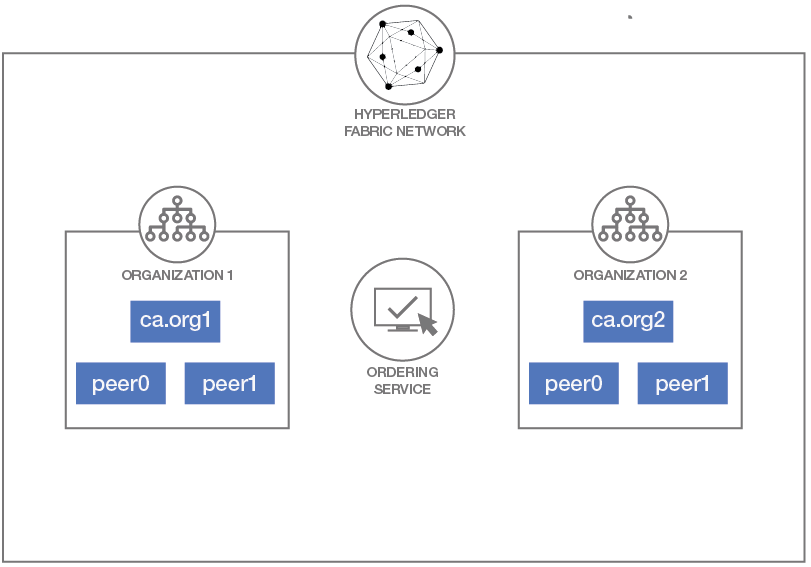
\includegraphics[width=(\textwidth),keepaspectratio]{img/my_org.png}
                \caption{Application topology}
                \label{obr 1.2.1}
            \end{center}
        \end{minipage}
    \end{center}
\end{figure}
\newpage

